\documentclass[twoside]{book}

% Packages required by doxygen
\usepackage{calc}
\usepackage{doxygen}
\usepackage{graphicx}
\usepackage[utf8]{inputenc}
\usepackage{makeidx}
\usepackage{multicol}
\usepackage{multirow}
\usepackage{textcomp}
\usepackage[table]{xcolor}

% NLS support packages
\usepackage[spanish]{babel}
% Font selection
\usepackage[T1]{fontenc}
\usepackage{mathptmx}
\usepackage[scaled=.90]{helvet}
\usepackage{courier}
\usepackage{amssymb}
\usepackage{sectsty}
\renewcommand{\familydefault}{\sfdefault}
\allsectionsfont{%
  \fontseries{bc}\selectfont%
  \color{darkgray}%
}
\renewcommand{\DoxyLabelFont}{%
  \fontseries{bc}\selectfont%
  \color{darkgray}%
}

% Page & text layout
\usepackage{geometry}
\geometry{%
  a4paper,%
  top=2.5cm,%
  bottom=2.5cm,%
  left=2.5cm,%
  right=2.5cm%
}
\tolerance=750
\hfuzz=15pt
\hbadness=750
\setlength{\emergencystretch}{15pt}
\setlength{\parindent}{0cm}
\setlength{\parskip}{0.2cm}
\makeatletter
\renewcommand{\paragraph}{%
  \@startsection{paragraph}{4}{0ex}{-1.0ex}{1.0ex}{%
    \normalfont\normalsize\bfseries\SS@parafont%
  }%
}
\renewcommand{\subparagraph}{%
  \@startsection{subparagraph}{5}{0ex}{-1.0ex}{1.0ex}{%
    \normalfont\normalsize\bfseries\SS@subparafont%
  }%
}
\makeatother

% Headers & footers
\usepackage{fancyhdr}
\pagestyle{fancyplain}
\fancyhead[LE]{\fancyplain{}{\bfseries\thepage}}
\fancyhead[CE]{\fancyplain{}{}}
\fancyhead[RE]{\fancyplain{}{\bfseries\leftmark}}
\fancyhead[LO]{\fancyplain{}{\bfseries\rightmark}}
\fancyhead[CO]{\fancyplain{}{}}
\fancyhead[RO]{\fancyplain{}{\bfseries\thepage}}
\fancyfoot[LE]{\fancyplain{}{}}
\fancyfoot[CE]{\fancyplain{}{}}
\fancyfoot[RE]{\fancyplain{}{\bfseries\scriptsize Generado el Domingo, 8 de Diciembre de 2013 19:57:07 para Practica de PRO2. Gestion de revistas cientificas. por Doxygen }}
\fancyfoot[LO]{\fancyplain{}{\bfseries\scriptsize Generado el Domingo, 8 de Diciembre de 2013 19:57:07 para Practica de PRO2. Gestion de revistas cientificas. por Doxygen }}
\fancyfoot[CO]{\fancyplain{}{}}
\fancyfoot[RO]{\fancyplain{}{}}
\renewcommand{\footrulewidth}{0.4pt}
\renewcommand{\chaptermark}[1]{%
  \markboth{#1}{}%
}
\renewcommand{\sectionmark}[1]{%
  \markright{\thesection\ #1}%
}

% Indices & bibliography
\usepackage{natbib}
\usepackage[titles]{tocloft}
\setcounter{tocdepth}{3}
\setcounter{secnumdepth}{5}
\makeindex

% Hyperlinks (required, but should be loaded last)
\usepackage{ifpdf}
\ifpdf
  \usepackage[pdftex,pagebackref=true]{hyperref}
\else
  \usepackage[ps2pdf,pagebackref=true]{hyperref}
\fi
\hypersetup{%
  colorlinks=true,%
  linkcolor=blue,%
  citecolor=blue,%
  unicode%
}

% Custom commands
\newcommand{\clearemptydoublepage}{%
  \newpage{\pagestyle{empty}\cleardoublepage}%
}


%===== C O N T E N T S =====

\begin{document}

% Titlepage & ToC
\hypersetup{pageanchor=false}
\pagenumbering{roman}
\begin{titlepage}
\vspace*{7cm}
\begin{center}%
{\Large Practica de P\-R\-O2. Gestion de revistas cientificas. \\[1ex]\large version dic-\/2013 }\\
\vspace*{1cm}
{\large Generado por Doxygen 1.8.4}\\
\vspace*{0.5cm}
{\small Domingo, 8 de Diciembre de 2013 19:57:07}\\
\end{center}
\end{titlepage}
\clearemptydoublepage
\tableofcontents
\clearemptydoublepage
\pagenumbering{arabic}
\hypersetup{pageanchor=true}

%--- Begin generated contents ---
\chapter{Índice de clases}
\section{Lista de clases}
Lista de las clases, estructuras, uniones e interfaces con una breve descripción\-:\begin{DoxyCompactList}
\item\contentsline{section}{\hyperlink{struct_biblioteca_1_1_a1}{Biblioteca\-::\-A1} \\*\hyperlink{struct_biblioteca_1_1_a1}{A1} es un struct que contiene por un lado una lista de revistas (L1) y por otro lado una lista de pairs de strings (L2) }{\pageref{struct_biblioteca_1_1_a1}}{}
\item\contentsline{section}{\hyperlink{class_biblioteca}{Biblioteca} \\*Representa una coleccion de revistas }{\pageref{class_biblioteca}}{}
\item\contentsline{section}{\hyperlink{class_esquema}{Esquema} \\*Representa la organizacion de la coleccion de revistas }{\pageref{class_esquema}}{}
\item\contentsline{section}{\hyperlink{class_revista}{Revista} \\*Representa el cojunto de caracteristicas y operaciones de las revistas }{\pageref{class_revista}}{}
\end{DoxyCompactList}

\chapter{Indice de archivos}
\section{Lista de archivos}
Lista de todos los archivos con descripciones breves\-:\begin{DoxyCompactList}
\item\contentsline{section}{\hyperlink{_biblioteca_8cpp}{Biblioteca.\-cpp} }{\pageref{_biblioteca_8cpp}}{}
\item\contentsline{section}{\hyperlink{_biblioteca_8hpp}{Biblioteca.\-hpp} \\*Especificacion de la clase \hyperlink{class_biblioteca}{Biblioteca} }{\pageref{_biblioteca_8hpp}}{}
\item\contentsline{section}{\hyperlink{_esquema_8cpp}{Esquema.\-cpp} }{\pageref{_esquema_8cpp}}{}
\item\contentsline{section}{\hyperlink{_esquema_8hpp}{Esquema.\-hpp} \\*Especificacion de la clase \hyperlink{class_esquema}{Esquema} }{\pageref{_esquema_8hpp}}{}
\item\contentsline{section}{\hyperlink{pro2_8cpp}{pro2.\-cpp} }{\pageref{pro2_8cpp}}{}
\item\contentsline{section}{\hyperlink{_revista_8cpp}{Revista.\-cpp} }{\pageref{_revista_8cpp}}{}
\item\contentsline{section}{\hyperlink{_revista_8hpp}{Revista.\-hpp} \\*Especificacion de la clase \hyperlink{class_revista}{Revista} }{\pageref{_revista_8hpp}}{}
\end{DoxyCompactList}

\chapter{Documentación de las clases}
\hypertarget{struct_biblioteca_1_1_a1}{\section{Referencia de la Estructura Biblioteca\-:\-:A1}
\label{struct_biblioteca_1_1_a1}\index{Biblioteca\-::\-A1@{Biblioteca\-::\-A1}}
}


\hyperlink{struct_biblioteca_1_1_a1}{A1} es un struct que contiene por un lado una lista de revistas (L1) y por otro lado una lista de pairs de strings (L2)  


\subsection*{Atributos públicos}
\begin{DoxyCompactItemize}
\item 
list$<$ \hyperlink{class_revista}{Revista} $>$ \hyperlink{struct_biblioteca_1_1_a1_a5aa560f4da33b9157b1b69c974de59c2}{L1}
\begin{DoxyCompactList}\small\item\em Lista de revistas. \end{DoxyCompactList}\item 
list$<$ pair$<$ string, string $>$ $>$ \hyperlink{struct_biblioteca_1_1_a1_a8463b0647409ec910cfdbf7fdaaa86b2}{L2}
\begin{DoxyCompactList}\small\item\em Lista de pairs de strings. \end{DoxyCompactList}\end{DoxyCompactItemize}


\subsection{Descripción detallada}
\hyperlink{struct_biblioteca_1_1_a1}{A1} es un struct que contiene por un lado una lista de revistas (L1) y por otro lado una lista de pairs de strings (L2) 

Definición en la línea 25 del archivo Biblioteca.\-hpp.



\subsection{Documentación de los datos miembro}
\hypertarget{struct_biblioteca_1_1_a1_a5aa560f4da33b9157b1b69c974de59c2}{\index{Biblioteca\-::\-A1@{Biblioteca\-::\-A1}!L1@{L1}}
\index{L1@{L1}!Biblioteca::A1@{Biblioteca\-::\-A1}}
\subsubsection[{L1}]{\setlength{\rightskip}{0pt plus 5cm}list$<${\bf Revista}$>$ Biblioteca\-::\-A1\-::\-L1}}\label{struct_biblioteca_1_1_a1_a5aa560f4da33b9157b1b69c974de59c2}


Lista de revistas. 

Ordenada por orden alfabetico segin el area tematica y, dentro de cada area, por titulo de revista, en el cual esta clasificada cada \hyperlink{class_revista}{Revista} segun el criterio de clasificacion 1. 

Definición en la línea 29 del archivo Biblioteca.\-hpp.

\hypertarget{struct_biblioteca_1_1_a1_a8463b0647409ec910cfdbf7fdaaa86b2}{\index{Biblioteca\-::\-A1@{Biblioteca\-::\-A1}!L2@{L2}}
\index{L2@{L2}!Biblioteca::A1@{Biblioteca\-::\-A1}}
\subsubsection[{L2}]{\setlength{\rightskip}{0pt plus 5cm}list$<$pair$<$string, string$>$ $>$ Biblioteca\-::\-A1\-::\-L2}}\label{struct_biblioteca_1_1_a1_a8463b0647409ec910cfdbf7fdaaa86b2}


Lista de pairs de strings. 

Ordenada por orden alfabetico segun el area tematica y, dentro de cada area, por titulo de revista, en el cual esta clasificada cada \hyperlink{class_revista}{Revista} segun el criterio de clasificacion 2. 

Definición en la línea 33 del archivo Biblioteca.\-hpp.



La documentación para esta estructura fue generada a partir del siguiente fichero\-:\begin{DoxyCompactItemize}
\item 
\hyperlink{_biblioteca_8hpp}{Biblioteca.\-hpp}\end{DoxyCompactItemize}

\hypertarget{class_biblioteca}{\section{Referencia de la Clase Biblioteca}
\label{class_biblioteca}\index{Biblioteca@{Biblioteca}}
}


Representa una coleccion de revistas.  


\subsection*{Clases}
\begin{DoxyCompactItemize}
\item 
struct \hyperlink{struct_biblioteca_1_1_a1}{A1}
\begin{DoxyCompactList}\small\item\em \hyperlink{struct_biblioteca_1_1_a1}{A1} es un struct que contiene por un lado una lista de revistas (L1) y por otro lado una lista de pairs de strings (L2) \end{DoxyCompactList}\end{DoxyCompactItemize}
\subsection*{Métodos públicos}
\begin{DoxyCompactItemize}
\item 
\hyperlink{class_biblioteca_a021f69adcc57a5d04e6e12532a684e2b}{Biblioteca} (int N)
\begin{DoxyCompactList}\small\item\em Creadora por defecto. \end{DoxyCompactList}\item 
\hyperlink{class_biblioteca_ae3f55e8952ed4bdddb82ece48c52f6c0}{$\sim$\-Biblioteca} ()
\begin{DoxyCompactList}\small\item\em Destructora por defecto. \end{DoxyCompactList}\item 
void \hyperlink{class_biblioteca_a3a699f219da645b8c461d1d07dbf6c76}{alta\-\_\-revista} (\hyperlink{class_revista}{Revista} \&r, int N)
\begin{DoxyCompactList}\small\item\em Anade la \hyperlink{class_revista}{Revista} r a la \hyperlink{class_biblioteca}{Biblioteca}. \end{DoxyCompactList}\item 
void \hyperlink{class_biblioteca_a3a5acce11e50bd1c262dabe293567b48}{baja\-\_\-revista} (const string \&s)
\begin{DoxyCompactList}\small\item\em Elimina la \hyperlink{class_revista}{Revista} que tiene por nombre s de la \hyperlink{class_biblioteca}{Biblioteca}. \end{DoxyCompactList}\item 
void \hyperlink{class_biblioteca_a44e062939e33e5da4743da5197b971f7}{consultar\-\_\-revista} (const string \&s, \hyperlink{class_revista}{Revista} \&r, int \&i, bool \&b) const 
\begin{DoxyCompactList}\small\item\em Consulta la informacion de la \hyperlink{class_revista}{Revista} que tiene por nombre s. \end{DoxyCompactList}\item 
void \hyperlink{class_biblioteca_a1560e54ae8e81b7c0190b636278af7b5}{listar\-\_\-revistas} (int N, int criterio)
\begin{DoxyCompactList}\small\item\em Operacion de escritura. \end{DoxyCompactList}\end{DoxyCompactItemize}
\subsection*{Métodos privados}
\begin{DoxyCompactItemize}
\item 
void \hyperlink{class_biblioteca_a01cd1e76edd489bdfc49f112129860ba}{eliminar\-\_\-revista} (const string \&s, bool \&eliminada, int i)
\begin{DoxyCompactList}\small\item\em Elimina la \hyperlink{class_revista}{Revista} que tiene por nombre s de la \hyperlink{class_biblioteca}{Biblioteca}. \end{DoxyCompactList}\end{DoxyCompactItemize}
\subsection*{Atributos privados}
\begin{DoxyCompactItemize}
\item 
vector$<$ \hyperlink{struct_biblioteca_1_1_a1}{A1} $>$ \hyperlink{class_biblioteca_a83688a3fd707fd8671178e82d7c53f6e}{biblioteca}
\begin{DoxyCompactList}\small\item\em biblioteca es un vector de \hyperlink{struct_biblioteca_1_1_a1}{A1} \end{DoxyCompactList}\end{DoxyCompactItemize}


\subsection{Descripción detallada}
Representa una coleccion de revistas. 

Definición en la línea 19 del archivo Biblioteca.\-hpp.



\subsection{Documentación del constructor y destructor}
\hypertarget{class_biblioteca_a021f69adcc57a5d04e6e12532a684e2b}{\index{Biblioteca@{Biblioteca}!Biblioteca@{Biblioteca}}
\index{Biblioteca@{Biblioteca}!Biblioteca@{Biblioteca}}
\subsubsection[{Biblioteca}]{\setlength{\rightskip}{0pt plus 5cm}Biblioteca\-::\-Biblioteca (
\begin{DoxyParamCaption}
\item[{int}]{N}
\end{DoxyParamCaption}
)}}\label{class_biblioteca_a021f69adcc57a5d04e6e12532a684e2b}


Creadora por defecto. 

Se ejecuta automaticamente al declarar una \hyperlink{class_biblioteca}{Biblioteca}.

\begin{DoxyPrecond}{Precondición}
cierto 
\end{DoxyPrecond}
\begin{DoxyPostcond}{Postcondición}
El resultado es una \hyperlink{class_biblioteca}{Biblioteca} vacia de tamano N. 
\end{DoxyPostcond}


Definición en la línea 3 del archivo Biblioteca.\-cpp.


\begin{DoxyCode}
3                            \{
4     \hyperlink{class_biblioteca_a83688a3fd707fd8671178e82d7c53f6e}{biblioteca} = vector<A1> (N);
5 \}
\end{DoxyCode}
\hypertarget{class_biblioteca_ae3f55e8952ed4bdddb82ece48c52f6c0}{\index{Biblioteca@{Biblioteca}!$\sim$\-Biblioteca@{$\sim$\-Biblioteca}}
\index{$\sim$\-Biblioteca@{$\sim$\-Biblioteca}!Biblioteca@{Biblioteca}}
\subsubsection[{$\sim$\-Biblioteca}]{\setlength{\rightskip}{0pt plus 5cm}Biblioteca\-::$\sim$\-Biblioteca (
\begin{DoxyParamCaption}
{}
\end{DoxyParamCaption}
)}}\label{class_biblioteca_ae3f55e8952ed4bdddb82ece48c52f6c0}


Destructora por defecto. 



Definición en la línea 7 del archivo Biblioteca.\-cpp.


\begin{DoxyCode}
7                         \{
8 \}
\end{DoxyCode}


\subsection{Documentación de las funciones miembro}
\hypertarget{class_biblioteca_a3a699f219da645b8c461d1d07dbf6c76}{\index{Biblioteca@{Biblioteca}!alta\-\_\-revista@{alta\-\_\-revista}}
\index{alta\-\_\-revista@{alta\-\_\-revista}!Biblioteca@{Biblioteca}}
\subsubsection[{alta\-\_\-revista}]{\setlength{\rightskip}{0pt plus 5cm}void Biblioteca\-::alta\-\_\-revista (
\begin{DoxyParamCaption}
\item[{{\bf Revista} \&}]{r, }
\item[{int}]{N}
\end{DoxyParamCaption}
)}}\label{class_biblioteca_a3a699f219da645b8c461d1d07dbf6c76}


Anade la \hyperlink{class_revista}{Revista} r a la \hyperlink{class_biblioteca}{Biblioteca}. 

\begin{DoxyPrecond}{Precondición}
La \hyperlink{class_revista}{Revista} no esta en la \hyperlink{class_biblioteca}{Biblioteca}. 
\end{DoxyPrecond}
\begin{DoxyPostcond}{Postcondición}
La \hyperlink{class_revista}{Revista} r, con indice de calidad N, pasa a formar parte de la \hyperlink{class_biblioteca}{Biblioteca}. 
\end{DoxyPostcond}


Definición en la línea 10 del archivo Biblioteca.\-cpp.


\begin{DoxyCode}
10                                                \{
11     list<Revista>::iterator it = \hyperlink{class_biblioteca_a83688a3fd707fd8671178e82d7c53f6e}{biblioteca}[N-1].L1.begin();
12     \textcolor{keywordflow}{if} (\hyperlink{class_biblioteca_a83688a3fd707fd8671178e82d7c53f6e}{biblioteca}[N-1].L1.empty()) \hyperlink{class_biblioteca_a83688a3fd707fd8671178e82d7c53f6e}{biblioteca}[N-1].L1.insert(it,r);
13     \textcolor{keywordflow}{else}\{
14   \textcolor{keywordtype}{bool} anadida = \textcolor{keyword}{false};
15   \textcolor{keywordflow}{while} (it != \hyperlink{class_biblioteca_a83688a3fd707fd8671178e82d7c53f6e}{biblioteca}[N-1].L1.end() and not anadida)\{
16       \textcolor{keywordflow}{if} (r.\hyperlink{class_revista_ae069d5a6c3e1c7996388505b4fde5a53}{cons\_c1}() == (*it).cons\_c1())\{
17     \textcolor{keywordflow}{if} (r.\hyperlink{class_revista_a2739f78a2d67490287421da71b5ea2f6}{cons\_nombre}() < (*it).cons\_nombre())\{
18         \hyperlink{class_biblioteca_a83688a3fd707fd8671178e82d7c53f6e}{biblioteca}[N-1].L1.insert(it,r);
19         anadida = \textcolor{keyword}{true};
20     \}
21     \textcolor{keywordflow}{else} ++it;
22       \}
23       \textcolor{keywordflow}{else} \textcolor{keywordflow}{if} (r.\hyperlink{class_revista_ae069d5a6c3e1c7996388505b4fde5a53}{cons\_c1}() < (*it).cons\_c1())\{
24     \hyperlink{class_biblioteca_a83688a3fd707fd8671178e82d7c53f6e}{biblioteca}[N-1].L1.insert(it,r);
25     anadida = \textcolor{keyword}{true};
26       \}
27       \textcolor{keywordflow}{else} ++it;
28   \}
29   \textcolor{keywordflow}{if} (not anadida) \hyperlink{class_biblioteca_a83688a3fd707fd8671178e82d7c53f6e}{biblioteca}[N-1].L1.insert(it,r);
30     \}
31     list<pair<string, string> >::iterator it2 = \hyperlink{class_biblioteca_a83688a3fd707fd8671178e82d7c53f6e}{biblioteca}[N-1].L2.begin();
32     pair<string, string> aux;
33     aux.first = r.\hyperlink{class_revista_a2739f78a2d67490287421da71b5ea2f6}{cons\_nombre}();
34     aux.second = r.\hyperlink{class_revista_a56072f31d4ee209c961cf3495a6a0687}{cons\_c2}();
35     \textcolor{keywordflow}{if} (\hyperlink{class_biblioteca_a83688a3fd707fd8671178e82d7c53f6e}{biblioteca}[N-1].L2.empty()) \hyperlink{class_biblioteca_a83688a3fd707fd8671178e82d7c53f6e}{biblioteca}[N-1].L2.insert(it2,aux);
36     \textcolor{keywordflow}{else}\{
37   \textcolor{keywordtype}{bool} anadida2 = \textcolor{keyword}{false};
38   \textcolor{keywordflow}{while} (it2 != \hyperlink{class_biblioteca_a83688a3fd707fd8671178e82d7c53f6e}{biblioteca}[N-1].L2.end() and not anadida2)\{
39       \textcolor{keywordflow}{if} (r.\hyperlink{class_revista_a56072f31d4ee209c961cf3495a6a0687}{cons\_c2}() == (*it2).second)\{
40     \textcolor{keywordflow}{if} (r.\hyperlink{class_revista_a2739f78a2d67490287421da71b5ea2f6}{cons\_nombre}() < (*it2).first)\{
41         \hyperlink{class_biblioteca_a83688a3fd707fd8671178e82d7c53f6e}{biblioteca}[N-1].L2.insert(it2,aux);
42         anadida2 = \textcolor{keyword}{true};
43     \}
44     \textcolor{keywordflow}{else} ++it2;
45       \}
46       \textcolor{keywordflow}{else} \textcolor{keywordflow}{if} (r.\hyperlink{class_revista_a56072f31d4ee209c961cf3495a6a0687}{cons\_c2}() < (*it2).second)\{
47     \hyperlink{class_biblioteca_a83688a3fd707fd8671178e82d7c53f6e}{biblioteca}[N-1].L2.insert(it2,aux);
48     anadida2 = \textcolor{keyword}{true};
49       \}
50       \textcolor{keywordflow}{else} ++it2;
51   \}
52   \textcolor{keywordflow}{if} (not anadida2) \hyperlink{class_biblioteca_a83688a3fd707fd8671178e82d7c53f6e}{biblioteca}[N-1].L2.insert(\hyperlink{class_biblioteca_a83688a3fd707fd8671178e82d7c53f6e}{biblioteca}[N-1].L2.end(),aux); 
53     \}
54 \}
\end{DoxyCode}
\hypertarget{class_biblioteca_a3a5acce11e50bd1c262dabe293567b48}{\index{Biblioteca@{Biblioteca}!baja\-\_\-revista@{baja\-\_\-revista}}
\index{baja\-\_\-revista@{baja\-\_\-revista}!Biblioteca@{Biblioteca}}
\subsubsection[{baja\-\_\-revista}]{\setlength{\rightskip}{0pt plus 5cm}void Biblioteca\-::baja\-\_\-revista (
\begin{DoxyParamCaption}
\item[{const string \&}]{s}
\end{DoxyParamCaption}
)}}\label{class_biblioteca_a3a5acce11e50bd1c262dabe293567b48}


Elimina la \hyperlink{class_revista}{Revista} que tiene por nombre s de la \hyperlink{class_biblioteca}{Biblioteca}. 

\begin{DoxyPrecond}{Precondición}
La \hyperlink{class_revista}{Revista}, que tiene por nombre s, esta en la biblioteca. 
\end{DoxyPrecond}
\begin{DoxyPostcond}{Postcondición}
La \hyperlink{class_revista}{Revista}, que tiene por nombre s, deja de formar parte de la \hyperlink{class_biblioteca}{Biblioteca}. 
\end{DoxyPostcond}


Definición en la línea 56 del archivo Biblioteca.\-cpp.


\begin{DoxyCode}
56                                              \{
57     \textcolor{keywordtype}{bool} eliminada = \textcolor{keyword}{false};
58     \textcolor{keywordtype}{int} i = 0;
59     \textcolor{keywordflow}{while} (i < \hyperlink{class_biblioteca_a83688a3fd707fd8671178e82d7c53f6e}{biblioteca}.size() and not eliminada)\{
60   \hyperlink{class_biblioteca_a01cd1e76edd489bdfc49f112129860ba}{eliminar\_revista}(s, eliminada, i);
61   \textcolor{keywordflow}{if} (not eliminada) ++i;
62     \}
63     \textcolor{keywordtype}{bool} eliminada2 = \textcolor{keyword}{false};
64     list<pair<string, string> >::iterator it2 = \hyperlink{class_biblioteca_a83688a3fd707fd8671178e82d7c53f6e}{biblioteca}[i].L2.begin();
65     \textcolor{keywordflow}{while} (it2 != \hyperlink{class_biblioteca_a83688a3fd707fd8671178e82d7c53f6e}{biblioteca}[i].L2.end() and not eliminada2)\{
66   \textcolor{keywordflow}{if} ((*it2).first == s)\{
67       it2 = \hyperlink{class_biblioteca_a83688a3fd707fd8671178e82d7c53f6e}{biblioteca}[i].L2.erase(it2);      
68       eliminada2 = \textcolor{keyword}{true};
69   \}
70   \textcolor{keywordflow}{else} ++it2;
71     \}
72 \}
\end{DoxyCode}
\hypertarget{class_biblioteca_a44e062939e33e5da4743da5197b971f7}{\index{Biblioteca@{Biblioteca}!consultar\-\_\-revista@{consultar\-\_\-revista}}
\index{consultar\-\_\-revista@{consultar\-\_\-revista}!Biblioteca@{Biblioteca}}
\subsubsection[{consultar\-\_\-revista}]{\setlength{\rightskip}{0pt plus 5cm}void Biblioteca\-::consultar\-\_\-revista (
\begin{DoxyParamCaption}
\item[{const string \&}]{s, }
\item[{{\bf Revista} \&}]{r, }
\item[{int \&}]{i, }
\item[{bool \&}]{b}
\end{DoxyParamCaption}
) const}}\label{class_biblioteca_a44e062939e33e5da4743da5197b971f7}


Consulta la informacion de la \hyperlink{class_revista}{Revista} que tiene por nombre s. 

\begin{DoxyPrecond}{Precondición}
Cierto. 
\end{DoxyPrecond}
\begin{DoxyPostcond}{Postcondición}
El resultado indica si la revista con nombre s se encuentra o no en la \hyperlink{class_biblioteca}{Biblioteca}. En caso afirmativo, devuelve toda la informacion que contiene una \hyperlink{class_revista}{Revista} junto su indice de calidad. 
\end{DoxyPostcond}


Definición en la línea 85 del archivo Biblioteca.\-cpp.


\begin{DoxyCode}
85                                                                                           \{
86     \hyperlink{class_revista}{Revista} aux;
87     \textcolor{keywordflow}{while} (i < \hyperlink{class_biblioteca_a83688a3fd707fd8671178e82d7c53f6e}{biblioteca}.size() and not existe)\{
88         list<Revista>::const\_iterator it = \hyperlink{class_biblioteca_a83688a3fd707fd8671178e82d7c53f6e}{biblioteca}[i].L1.begin();
89   \textcolor{keywordflow}{while} (it != \hyperlink{class_biblioteca_a83688a3fd707fd8671178e82d7c53f6e}{biblioteca}[i].L1.end() and not existe)\{
90             \textcolor{keywordflow}{if}((*it).cons\_nombre() == s)\{
91     aux = (*it);
92     existe = \textcolor{keyword}{true};
93       \}
94       \textcolor{keywordflow}{else} ++it;
95   \}
96   ++i;
97    \}
98    r = aux;
99 \}
\end{DoxyCode}
\hypertarget{class_biblioteca_a1560e54ae8e81b7c0190b636278af7b5}{\index{Biblioteca@{Biblioteca}!listar\-\_\-revistas@{listar\-\_\-revistas}}
\index{listar\-\_\-revistas@{listar\-\_\-revistas}!Biblioteca@{Biblioteca}}
\subsubsection[{listar\-\_\-revistas}]{\setlength{\rightskip}{0pt plus 5cm}void Biblioteca\-::listar\-\_\-revistas (
\begin{DoxyParamCaption}
\item[{int}]{N, }
\item[{int}]{criterio}
\end{DoxyParamCaption}
)}}\label{class_biblioteca_a1560e54ae8e81b7c0190b636278af7b5}


Operacion de escritura. 

\begin{DoxyPrecond}{Precondición}
cierto 
\end{DoxyPrecond}
\begin{DoxyPostcond}{Postcondición}
Dependiendo del indice de calidad (N) y el criterio a seguir, se escribiran las revistas de indice N junto a su correspondiente area tematica segun el criterio a seguir, ordenadas en orden alfabetico de area y, dentro de cada area, por titulo de \hyperlink{class_revista}{Revista}, por el canal estandard de salida. 
\end{DoxyPostcond}


Definición en la línea 101 del archivo Biblioteca.\-cpp.


\begin{DoxyCode}
101                                                     \{
102     \textcolor{keywordflow}{if} (criterio == 1)\{
103   list<Revista>::const\_iterator it = \hyperlink{class_biblioteca_a83688a3fd707fd8671178e82d7c53f6e}{biblioteca}[N-1].L1.begin();
104   \textcolor{keywordflow}{while} (it != \hyperlink{class_biblioteca_a83688a3fd707fd8671178e82d7c53f6e}{biblioteca}[N-1].L1.end())\{
105       cout << (*it).cons\_c1() << \textcolor{stringliteral}{" "} << (*it).cons\_nombre() << endl;
106       ++it;
107   \}
108     \}
109     \textcolor{keywordflow}{else} \{
110   list<pair<string, string> >::const\_iterator it = \hyperlink{class_biblioteca_a83688a3fd707fd8671178e82d7c53f6e}{biblioteca}[N-1].L2.begin();
111   \textcolor{keywordflow}{while} (it != \hyperlink{class_biblioteca_a83688a3fd707fd8671178e82d7c53f6e}{biblioteca}[N-1].L2.end())\{
112       cout << (*it).second << \textcolor{stringliteral}{" "} << (*it).first << endl;
113       ++it;
114   \}
115     \}
116 \}\end{DoxyCode}
\hypertarget{class_biblioteca_a01cd1e76edd489bdfc49f112129860ba}{\index{Biblioteca@{Biblioteca}!eliminar\-\_\-revista@{eliminar\-\_\-revista}}
\index{eliminar\-\_\-revista@{eliminar\-\_\-revista}!Biblioteca@{Biblioteca}}
\subsubsection[{eliminar\-\_\-revista}]{\setlength{\rightskip}{0pt plus 5cm}void Biblioteca\-::eliminar\-\_\-revista (
\begin{DoxyParamCaption}
\item[{const string \&}]{s, }
\item[{bool \&}]{eliminada, }
\item[{int}]{i}
\end{DoxyParamCaption}
)\hspace{0.3cm}{\ttfamily [private]}}}\label{class_biblioteca_a01cd1e76edd489bdfc49f112129860ba}


Elimina la \hyperlink{class_revista}{Revista} que tiene por nombre s de la \hyperlink{class_biblioteca}{Biblioteca}. 

\begin{DoxyPrecond}{Precondición}
Cierto. 
\end{DoxyPrecond}
\begin{DoxyPostcond}{Postcondición}
La \hyperlink{class_revista}{Revista}, que tiene por nombre s, deja de formar parte de la \hyperlink{class_biblioteca}{Biblioteca} si eliminada es true. 
\end{DoxyPostcond}


Definición en la línea 74 del archivo Biblioteca.\-cpp.


\begin{DoxyCode}
74                                                                          \{
75     list<Revista>::iterator it = \hyperlink{class_biblioteca_a83688a3fd707fd8671178e82d7c53f6e}{biblioteca}[i].L1.begin();
76     \textcolor{keywordflow}{while} (it != \hyperlink{class_biblioteca_a83688a3fd707fd8671178e82d7c53f6e}{biblioteca}[i].L1.end() and not eliminada)\{
77   \textcolor{keywordflow}{if} ((*it).cons\_nombre() == s)\{
78       it = \hyperlink{class_biblioteca_a83688a3fd707fd8671178e82d7c53f6e}{biblioteca}[i].L1.erase(it);
79       eliminada = \textcolor{keyword}{true};
80   \}
81   \textcolor{keywordflow}{else} ++it;
82     \}
83 \}
\end{DoxyCode}


\subsection{Documentación de los datos miembro}
\hypertarget{class_biblioteca_a83688a3fd707fd8671178e82d7c53f6e}{\index{Biblioteca@{Biblioteca}!biblioteca@{biblioteca}}
\index{biblioteca@{biblioteca}!Biblioteca@{Biblioteca}}
\subsubsection[{biblioteca}]{\setlength{\rightskip}{0pt plus 5cm}vector$<${\bf A1}$>$ Biblioteca\-::biblioteca\hspace{0.3cm}{\ttfamily [private]}}}\label{class_biblioteca_a83688a3fd707fd8671178e82d7c53f6e}


biblioteca es un vector de \hyperlink{struct_biblioteca_1_1_a1}{A1} 



Definición en la línea 37 del archivo Biblioteca.\-hpp.



La documentación para esta clase fue generada a partir de los siguientes ficheros\-:\begin{DoxyCompactItemize}
\item 
\hyperlink{_biblioteca_8hpp}{Biblioteca.\-hpp}\item 
\hyperlink{_biblioteca_8cpp}{Biblioteca.\-cpp}\end{DoxyCompactItemize}

\hypertarget{class_esquema}{\section{Referencia de la Clase Esquema}
\label{class_esquema}\index{Esquema@{Esquema}}
}


Representa la organizacion de la coleccion de revistas.  


\subsection*{Métodos públicos}
\begin{DoxyCompactItemize}
\item 
\hyperlink{class_esquema_af1460486d823ed42510655affd487fa1}{Esquema} ()
\begin{DoxyCompactList}\small\item\em Creadora por defecto. \end{DoxyCompactList}\item 
\hyperlink{class_esquema_a35493f2aa427f0cea80f7ece50d22f6e}{$\sim$\-Esquema} ()
\begin{DoxyCompactList}\small\item\em Destructora por defecto. \end{DoxyCompactList}\item 
void \hyperlink{class_esquema_a2a237e94381f752b6f5cb582987b0570}{calcular\-\_\-c1} (\hyperlink{class_revista}{Revista} \&r) const 
\begin{DoxyCompactList}\small\item\em Calcula el area tematica en el cual esta clasificada la \hyperlink{class_revista}{Revista} r segun el criterio de clasificacion 1. \end{DoxyCompactList}\item 
void \hyperlink{class_esquema_a50c270ca5ba9dbd129fe047fb7a18363}{calcular\-\_\-c2} (\hyperlink{class_revista}{Revista} \&r) const 
\begin{DoxyCompactList}\small\item\em Calcula el area tematica en el cual esta clasificada la \hyperlink{class_revista}{Revista} r segun el criterio de clasificacion 2. \end{DoxyCompactList}\item 
void \hyperlink{class_esquema_ad6c7e82a2322bd19412efa51d2005ede}{leer\-\_\-esquema} ()
\begin{DoxyCompactList}\small\item\em Operacion de lectura. \end{DoxyCompactList}\end{DoxyCompactItemize}
\subsection*{Métodos privados estáticos}
\begin{DoxyCompactItemize}
\item 
static void \hyperlink{class_esquema_abf74b66701d3ab70316d8740cdd0bc25}{fusionar\-\_\-listas} (list$<$ string $>$ \&lista1, list$<$ string $>$ \&lista2)
\begin{DoxyCompactList}\small\item\em Añade los elementos de la lista2 a la lista1. \end{DoxyCompactList}\item 
static void \hyperlink{class_esquema_a77210c8349dc7dccbaa8224c2da4e50e}{auxcalcular\-\_\-c1} (\hyperlink{class_revista}{Revista} \&r, Arbre$<$ string $>$ \&\hyperlink{class_esquema_aee89f1d564d1951112b2f10a47f943aa}{a}, int altura\-\_\-inicial, int \&altura\-\_\-areatematica, list$<$ string $>$ \&lista, bool \&todas\-\_\-encontradas, string \&area\-\_\-tematica)
\begin{DoxyCompactList}\small\item\em Calcula el area tematica en el cual esta clasificada la \hyperlink{class_revista}{Revista} r segun el criterio de clasificacion 1. \end{DoxyCompactList}\item 
static pair$<$ bool, string $>$ \hyperlink{class_esquema_a1e863b6bd93430abe836d339bd7bcba7}{auxcalcular\-\_\-c2} (\hyperlink{class_revista}{Revista} \&r, Arbre$<$ string $>$ \&\hyperlink{class_esquema_aee89f1d564d1951112b2f10a47f943aa}{a})
\begin{DoxyCompactList}\small\item\em Calcula el area tematica en el cual esta clasificada la \hyperlink{class_revista}{Revista} r segun el criterio de clasificacion 2. \end{DoxyCompactList}\item 
static void \hyperlink{class_esquema_acdc1f43dae72e916d6baf7f53f973a21}{leer\-\_\-esquema2} (Arbre$<$ string $>$ \&\hyperlink{class_esquema_aee89f1d564d1951112b2f10a47f943aa}{a}, string marca)
\begin{DoxyCompactList}\small\item\em Operacion de lectura de un arbol de strings. \end{DoxyCompactList}\end{DoxyCompactItemize}
\subsection*{Atributos privados}
\begin{DoxyCompactItemize}
\item 
Arbre$<$ string $>$ \hyperlink{class_esquema_aee89f1d564d1951112b2f10a47f943aa}{a}
\begin{DoxyCompactList}\small\item\em Estructura de areas tematicas de la biblioteca. \end{DoxyCompactList}\end{DoxyCompactItemize}


\subsection{Descripción detallada}
Representa la organizacion de la coleccion de revistas. 

Definición en la línea 17 del archivo Esquema.\-hpp.



\subsection{Documentación del constructor y destructor}
\hypertarget{class_esquema_af1460486d823ed42510655affd487fa1}{\index{Esquema@{Esquema}!Esquema@{Esquema}}
\index{Esquema@{Esquema}!Esquema@{Esquema}}
\subsubsection[{Esquema}]{\setlength{\rightskip}{0pt plus 5cm}Esquema\-::\-Esquema (
\begin{DoxyParamCaption}
{}
\end{DoxyParamCaption}
)}}\label{class_esquema_af1460486d823ed42510655affd487fa1}


Creadora por defecto. 

Se ejecuta automaticamente al declarar un \hyperlink{class_esquema}{Esquema}.

\begin{DoxyPrecond}{Precondición}
cierto 
\end{DoxyPrecond}
\begin{DoxyPostcond}{Postcondición}
El resultado es un esquema vacio. 
\end{DoxyPostcond}


Definición en la línea 3 del archivo Esquema.\-cpp.


\begin{DoxyCode}
3                 \{
4 \}
\end{DoxyCode}
\hypertarget{class_esquema_a35493f2aa427f0cea80f7ece50d22f6e}{\index{Esquema@{Esquema}!$\sim$\-Esquema@{$\sim$\-Esquema}}
\index{$\sim$\-Esquema@{$\sim$\-Esquema}!Esquema@{Esquema}}
\subsubsection[{$\sim$\-Esquema}]{\setlength{\rightskip}{0pt plus 5cm}Esquema\-::$\sim$\-Esquema (
\begin{DoxyParamCaption}
{}
\end{DoxyParamCaption}
)}}\label{class_esquema_a35493f2aa427f0cea80f7ece50d22f6e}


Destructora por defecto. 



Definición en la línea 6 del archivo Esquema.\-cpp.


\begin{DoxyCode}
6                  \{
7 \}
\end{DoxyCode}


\subsection{Documentación de las funciones miembro}
\hypertarget{class_esquema_a2a237e94381f752b6f5cb582987b0570}{\index{Esquema@{Esquema}!calcular\-\_\-c1@{calcular\-\_\-c1}}
\index{calcular\-\_\-c1@{calcular\-\_\-c1}!Esquema@{Esquema}}
\subsubsection[{calcular\-\_\-c1}]{\setlength{\rightskip}{0pt plus 5cm}void Esquema\-::calcular\-\_\-c1 (
\begin{DoxyParamCaption}
\item[{{\bf Revista} \&}]{r}
\end{DoxyParamCaption}
) const}}\label{class_esquema_a2a237e94381f752b6f5cb582987b0570}


Calcula el area tematica en el cual esta clasificada la \hyperlink{class_revista}{Revista} r segun el criterio de clasificacion 1. 

\begin{DoxyPrecond}{Precondición}
Todas las palabras clave de la \hyperlink{class_revista}{Revista} r deben estar en \hyperlink{class_esquema}{Esquema}. 
\end{DoxyPrecond}
\begin{DoxyPostcond}{Postcondición}
Calcula y asigna el area tematica en el cual esta clasificada la \hyperlink{class_revista}{Revista} r segun el criterio de clasificacion 1. 
\end{DoxyPostcond}


Definición en la línea 9 del archivo Esquema.\-cpp.


\begin{DoxyCode}
9                                          \{
10     Arbre<string> copia(\hyperlink{class_esquema_aee89f1d564d1951112b2f10a47f943aa}{a});
11     list <string> lista;
12     \textcolor{keywordtype}{bool} todas\_encontradas;
13     \textcolor{keywordtype}{string} area\_tematica;
14     \textcolor{keywordtype}{int} altura\_inicial = 1;
15     \textcolor{keywordtype}{int} altura\_areatematica;
16     \hyperlink{class_esquema_a77210c8349dc7dccbaa8224c2da4e50e}{auxcalcular\_c1}(r, copia, altura\_inicial, altura\_areatematica, lista, todas\_encontradas, 
      area\_tematica);
17     r.\hyperlink{class_revista_a526d3f522dfdd299ddd7ef3d317c3101}{mod\_c1}(area\_tematica);
18 \}
\end{DoxyCode}
\hypertarget{class_esquema_a50c270ca5ba9dbd129fe047fb7a18363}{\index{Esquema@{Esquema}!calcular\-\_\-c2@{calcular\-\_\-c2}}
\index{calcular\-\_\-c2@{calcular\-\_\-c2}!Esquema@{Esquema}}
\subsubsection[{calcular\-\_\-c2}]{\setlength{\rightskip}{0pt plus 5cm}void Esquema\-::calcular\-\_\-c2 (
\begin{DoxyParamCaption}
\item[{{\bf Revista} \&}]{r}
\end{DoxyParamCaption}
) const}}\label{class_esquema_a50c270ca5ba9dbd129fe047fb7a18363}


Calcula el area tematica en el cual esta clasificada la \hyperlink{class_revista}{Revista} r segun el criterio de clasificacion 2. 

\begin{DoxyPrecond}{Precondición}
Todas las palabras clave de la \hyperlink{class_revista}{Revista} r deben estar en \hyperlink{class_esquema}{Esquema}. 
\end{DoxyPrecond}
\begin{DoxyPostcond}{Postcondición}
Calcula y asigna el area tematica en el cual esta clasificada la \hyperlink{class_revista}{Revista} r segun el criterio de clasificacion 2. 
\end{DoxyPostcond}


Definición en la línea 124 del archivo Esquema.\-cpp.


\begin{DoxyCode}
124                                          \{
125     pair<bool, string> aux;
126     Arbre<string> copia(\hyperlink{class_esquema_aee89f1d564d1951112b2f10a47f943aa}{a});
127     aux = \hyperlink{class_esquema_a1e863b6bd93430abe836d339bd7bcba7}{auxcalcular\_c2}(r, copia);
128     r.\hyperlink{class_revista_af48636e38adc7248ae7a2028e51bc9f2}{mod\_c2}(aux.second);
129 \}
\end{DoxyCode}
\hypertarget{class_esquema_ad6c7e82a2322bd19412efa51d2005ede}{\index{Esquema@{Esquema}!leer\-\_\-esquema@{leer\-\_\-esquema}}
\index{leer\-\_\-esquema@{leer\-\_\-esquema}!Esquema@{Esquema}}
\subsubsection[{leer\-\_\-esquema}]{\setlength{\rightskip}{0pt plus 5cm}void Esquema\-::leer\-\_\-esquema (
\begin{DoxyParamCaption}
{}
\end{DoxyParamCaption}
)}}\label{class_esquema_ad6c7e82a2322bd19412efa51d2005ede}


Operacion de lectura. 

\begin{DoxyPrecond}{Precondición}
Cierto 
\end{DoxyPrecond}
\begin{DoxyPostcond}{Postcondición}
a contiene el esquema leido por el canal estandard de entrada. 
\end{DoxyPostcond}


Definición en la línea 180 del archivo Esquema.\-cpp.


\begin{DoxyCode}
180                           \{
181    \hyperlink{class_esquema_acdc1f43dae72e916d6baf7f53f973a21}{leer\_esquema2}(\hyperlink{class_esquema_aee89f1d564d1951112b2f10a47f943aa}{a}, \textcolor{stringliteral}{"."});
182 \}\end{DoxyCode}
\hypertarget{class_esquema_abf74b66701d3ab70316d8740cdd0bc25}{\index{Esquema@{Esquema}!fusionar\-\_\-listas@{fusionar\-\_\-listas}}
\index{fusionar\-\_\-listas@{fusionar\-\_\-listas}!Esquema@{Esquema}}
\subsubsection[{fusionar\-\_\-listas}]{\setlength{\rightskip}{0pt plus 5cm}void Esquema\-::fusionar\-\_\-listas (
\begin{DoxyParamCaption}
\item[{list$<$ string $>$ \&}]{lista1, }
\item[{list$<$ string $>$ \&}]{lista2}
\end{DoxyParamCaption}
)\hspace{0.3cm}{\ttfamily [static]}, {\ttfamily [private]}}}\label{class_esquema_abf74b66701d3ab70316d8740cdd0bc25}


Añade los elementos de la lista2 a la lista1. 

\begin{DoxyPrecond}{Precondición}
cierto. 
\end{DoxyPrecond}
\begin{DoxyPostcond}{Postcondición}
La lista1 pasa a tener los elementos que ya tenia mas los de la lista2 sin repetir ninguno. 
\end{DoxyPostcond}


Definición en la línea 100 del archivo Esquema.\-cpp.


\begin{DoxyCode}
100                                                                        \{
101     list<string>::iterator it = lista2.begin();
102     \textcolor{keywordflow}{while} (it != lista2.end())\{
103   list<string>::iterator it2 = lista1.begin();
104   \textcolor{keywordflow}{if} (lista1.empty()) \{
105       it2 = lista1.end();
106       lista1.insert(it2,(*it));
107   \}
108   \textcolor{keywordflow}{else} \{
109       \textcolor{keywordtype}{bool} trobat = \textcolor{keyword}{false};
110       \textcolor{keywordflow}{while} (it2 != lista1.end() and not trobat)\{
111     \textcolor{keywordflow}{if} ((*it) == (*it2)) trobat = \textcolor{keyword}{true};
112     \textcolor{keywordflow}{else} \textcolor{keywordflow}{if} ((*it) < (*it2))\{
113         lista1.insert(it2,(*it));
114         trobat = \textcolor{keyword}{true};
115     \}
116     \textcolor{keywordflow}{else} ++it2;
117       \}
118       \textcolor{keywordflow}{if} (not trobat) lista1.insert(it2,(*it));
119   \}
120     ++it;
121     \}
122 \}
\end{DoxyCode}
\hypertarget{class_esquema_a77210c8349dc7dccbaa8224c2da4e50e}{\index{Esquema@{Esquema}!auxcalcular\-\_\-c1@{auxcalcular\-\_\-c1}}
\index{auxcalcular\-\_\-c1@{auxcalcular\-\_\-c1}!Esquema@{Esquema}}
\subsubsection[{auxcalcular\-\_\-c1}]{\setlength{\rightskip}{0pt plus 5cm}void Esquema\-::auxcalcular\-\_\-c1 (
\begin{DoxyParamCaption}
\item[{{\bf Revista} \&}]{r, }
\item[{Arbre$<$ string $>$ \&}]{a, }
\item[{int}]{altura\-\_\-inicial, }
\item[{int \&}]{altura\-\_\-areatematica, }
\item[{list$<$ string $>$ \&}]{lista, }
\item[{bool \&}]{todas\-\_\-encontradas, }
\item[{string \&}]{area\-\_\-tematica}
\end{DoxyParamCaption}
)\hspace{0.3cm}{\ttfamily [static]}, {\ttfamily [private]}}}\label{class_esquema_a77210c8349dc7dccbaa8224c2da4e50e}


Calcula el area tematica en el cual esta clasificada la \hyperlink{class_revista}{Revista} r segun el criterio de clasificacion 1. 

\begin{DoxyPrecond}{Precondición}
lista1 y lista2 son listas ordenadas alfabeticamente. 
\end{DoxyPrecond}
\begin{DoxyPostcond}{Postcondición}
El string area\-\_\-tematica pasa a tener el valor de el area tematica en el cual esta clasificada la \hyperlink{class_revista}{Revista} r segun el criterio de clasificacion 1. 
\end{DoxyPostcond}


Definición en la línea 20 del archivo Esquema.\-cpp.


\begin{DoxyCode}
20                                                                                                            
                                                                      \{
21     \textcolor{keywordtype}{string} raiz = \hyperlink{class_esquema_aee89f1d564d1951112b2f10a47f943aa}{a}.arrel();
22     todas\_encontradas = \textcolor{keyword}{false};
23     Arbre<string> a1, a2;
24     \hyperlink{class_esquema_aee89f1d564d1951112b2f10a47f943aa}{a}.fills(a1, a2);
25     \textcolor{keywordflow}{if} (a1.es\_buit() and a2.es\_buit())\{
26   \textcolor{keywordflow}{if} (r.\hyperlink{class_revista_aad8d277011c68f7acdeac6f3d47d28cb}{cons\_palabrasclave}(raiz))\{
27       list<string>::iterator it = lista.begin();
28       lista.insert(it, raiz);
29   \}
30   \textcolor{keywordflow}{if} (lista.size() == r.\hyperlink{class_revista_a69d99a64d3ef987db733b4f492c53db8}{cons\_numeropalabrasclave}())\{
31       todas\_encontradas = \textcolor{keyword}{true};
32       area\_tematica = raiz;
33       altura\_areatematica = altura\_inicial;
34   \}
35     \}
36     \textcolor{keywordflow}{else} \{
37   \textcolor{keywordtype}{bool} todas\_encontradas1, todas\_encontradas2;
38   \textcolor{keywordtype}{string} area\_tematica1, area\_tematica2;
39   \textcolor{keywordtype}{int} altura\_areatematica1, altura\_areatematica2;
40   list<string> lista1, lista2;
41   \textcolor{keywordflow}{if} (a1.es\_buit() and not a2.es\_buit())\{
42       \hyperlink{class_esquema_a77210c8349dc7dccbaa8224c2da4e50e}{auxcalcular\_c1}(r, a2, altura\_inicial+1, altura\_areatematica2, lista2, 
      todas\_encontradas2, area\_tematica2); 
43       todas\_encontradas1 = \textcolor{keyword}{false};
44   \}
45   \textcolor{keywordflow}{else} \textcolor{keywordflow}{if} (not a1.es\_buit() and a2.es\_buit())\{
46       \hyperlink{class_esquema_a77210c8349dc7dccbaa8224c2da4e50e}{auxcalcular\_c1}(r, a1, altura\_inicial+1, altura\_areatematica1, lista1, 
      todas\_encontradas1, area\_tematica1); 
47       todas\_encontradas2 = \textcolor{keyword}{false};
48   \}
49   \textcolor{keywordflow}{else} \textcolor{keywordflow}{if} (not a1.es\_buit() and not a2.es\_buit())\{
50       \hyperlink{class_esquema_a77210c8349dc7dccbaa8224c2da4e50e}{auxcalcular\_c1}(r, a2, altura\_inicial+1, altura\_areatematica2, lista2, 
      todas\_encontradas2, area\_tematica2);
51       \hyperlink{class_esquema_a77210c8349dc7dccbaa8224c2da4e50e}{auxcalcular\_c1}(r, a1, altura\_inicial+1, altura\_areatematica1, lista1, 
      todas\_encontradas1, area\_tematica1); 
52   \}
53   \textcolor{keywordflow}{if} (not todas\_encontradas1 and not todas\_encontradas2) \{
54       \hyperlink{class_esquema_abf74b66701d3ab70316d8740cdd0bc25}{fusionar\_listas}(lista1, lista2);
55       lista = lista1;
56       \textcolor{keywordflow}{if} (lista.size() == r.\hyperlink{class_revista_a69d99a64d3ef987db733b4f492c53db8}{cons\_numeropalabrasclave}())\{  
57     todas\_encontradas = \textcolor{keyword}{true};
58     area\_tematica = raiz;
59     altura\_areatematica = altura\_inicial;
60       \}
61       \textcolor{keywordflow}{else} todas\_encontradas = \textcolor{keyword}{false};
62   \}
63   \textcolor{keywordflow}{else} \textcolor{keywordflow}{if} (not todas\_encontradas1 and todas\_encontradas2) \{
64       todas\_encontradas = \textcolor{keyword}{true};
65       area\_tematica = area\_tematica2;
66       altura\_areatematica = altura\_areatematica2;
67   \}
68   \textcolor{keywordflow}{else} \textcolor{keywordflow}{if} (todas\_encontradas1 and not todas\_encontradas2) \{
69       todas\_encontradas = \textcolor{keyword}{true};
70       area\_tematica = area\_tematica1;
71       altura\_areatematica = altura\_areatematica1;
72   \}
73   \textcolor{keywordflow}{else} \{
74       \textcolor{keywordflow}{if} (altura\_areatematica1 == altura\_areatematica2) \{
75     \textcolor{keywordflow}{if} (area\_tematica1 < area\_tematica2) \{
76         todas\_encontradas = \textcolor{keyword}{true};
77         area\_tematica = area\_tematica1;
78         altura\_areatematica = altura\_areatematica1;
79     \}
80     \textcolor{keywordflow}{else} \{
81         todas\_encontradas = \textcolor{keyword}{true};
82         area\_tematica = area\_tematica2;
83         altura\_areatematica = altura\_areatematica2;
84     \}
85       \}
86       \textcolor{keywordflow}{else} \textcolor{keywordflow}{if} (altura\_areatematica1 > altura\_areatematica2) \{
87     todas\_encontradas = \textcolor{keyword}{true};
88     area\_tematica = area\_tematica1;
89     altura\_areatematica = altura\_areatematica1;
90       \}
91       \textcolor{keywordflow}{else} \{
92     todas\_encontradas = \textcolor{keyword}{true};
93     area\_tematica = area\_tematica2;
94     altura\_areatematica = altura\_areatematica2;
95       \}
96   \}
97     \}
98 \}
\end{DoxyCode}
\hypertarget{class_esquema_a1e863b6bd93430abe836d339bd7bcba7}{\index{Esquema@{Esquema}!auxcalcular\-\_\-c2@{auxcalcular\-\_\-c2}}
\index{auxcalcular\-\_\-c2@{auxcalcular\-\_\-c2}!Esquema@{Esquema}}
\subsubsection[{auxcalcular\-\_\-c2}]{\setlength{\rightskip}{0pt plus 5cm}pair$<$ bool, string $>$ Esquema\-::auxcalcular\-\_\-c2 (
\begin{DoxyParamCaption}
\item[{{\bf Revista} \&}]{r, }
\item[{Arbre$<$ string $>$ \&}]{a}
\end{DoxyParamCaption}
)\hspace{0.3cm}{\ttfamily [static]}, {\ttfamily [private]}}}\label{class_esquema_a1e863b6bd93430abe836d339bd7bcba7}


Calcula el area tematica en el cual esta clasificada la \hyperlink{class_revista}{Revista} r segun el criterio de clasificacion 2. 

\begin{DoxyPrecond}{Precondición}
cierto. 
\end{DoxyPrecond}
\begin{DoxyPostcond}{Postcondición}
El primer componente del resultado indica si hemos encontrado una palabra clave de r; el segundo es el nombre de la area tematica en el cual esta clasificada la revista r segun el criterio de clasificacion 2. 
\end{DoxyPostcond}


Definición en la línea 131 del archivo Esquema.\-cpp.


\begin{DoxyCode}
131                                                                       \{
132     \textcolor{keywordtype}{string} raiz = \hyperlink{class_esquema_aee89f1d564d1951112b2f10a47f943aa}{a}.arrel();
133     pair<bool, string> aux, aux1, aux2;
134     aux.first = \textcolor{keyword}{false};
135     Arbre<string> a1, a2;
136     \hyperlink{class_esquema_aee89f1d564d1951112b2f10a47f943aa}{a}.fills(a1, a2);
137     \textcolor{keywordflow}{if} (a1.es\_buit() and a2.es\_buit())\{
138   \textcolor{keywordflow}{if} (r.\hyperlink{class_revista_aad8d277011c68f7acdeac6f3d47d28cb}{cons\_palabrasclave}(raiz))\{
139       aux.second = raiz;
140       aux.first = \textcolor{keyword}{true};
141   \}
142   \textcolor{keywordflow}{else} aux.first = \textcolor{keyword}{false};
143     \}
144     \textcolor{keywordflow}{else} \{
145   \textcolor{keywordflow}{if} (not a1.es\_buit() and not a2.es\_buit())\{
146       aux1 = \hyperlink{class_esquema_a1e863b6bd93430abe836d339bd7bcba7}{auxcalcular\_c2}(r, a1);
147       aux2 = \hyperlink{class_esquema_a1e863b6bd93430abe836d339bd7bcba7}{auxcalcular\_c2}(r, a2);
148   \}
149   \textcolor{keywordflow}{else} \textcolor{keywordflow}{if} (not a1.es\_buit() and a2.es\_buit())\{
150       aux1 = \hyperlink{class_esquema_a1e863b6bd93430abe836d339bd7bcba7}{auxcalcular\_c2}(r, a1);
151       aux2.first = \textcolor{keyword}{false};
152   \}
153   \textcolor{keywordflow}{else} \textcolor{keywordflow}{if} (a1.es\_buit() and not a2.es\_buit())\{
154       aux2 = \hyperlink{class_esquema_a1e863b6bd93430abe836d339bd7bcba7}{auxcalcular\_c2}(r, a2);
155       aux1.first = \textcolor{keyword}{false};
156   \}
157   \textcolor{keywordflow}{if} (not aux1.first and not aux2.first) aux.first = \textcolor{keyword}{false};
158   \textcolor{keywordflow}{else} \textcolor{keywordflow}{if} (aux1.first and not aux2.first) aux = aux1;
159   \textcolor{keywordflow}{else} \textcolor{keywordflow}{if} (not aux1.first and aux2.first) aux = aux2;
160   \textcolor{keywordflow}{else} \{
161       aux.second = raiz;
162       aux.first = \textcolor{keyword}{true};
163   \}
164     \}
165     \textcolor{keywordflow}{return} aux;
166 \}
\end{DoxyCode}
\hypertarget{class_esquema_acdc1f43dae72e916d6baf7f53f973a21}{\index{Esquema@{Esquema}!leer\-\_\-esquema2@{leer\-\_\-esquema2}}
\index{leer\-\_\-esquema2@{leer\-\_\-esquema2}!Esquema@{Esquema}}
\subsubsection[{leer\-\_\-esquema2}]{\setlength{\rightskip}{0pt plus 5cm}void Esquema\-::leer\-\_\-esquema2 (
\begin{DoxyParamCaption}
\item[{Arbre$<$ string $>$ \&}]{a, }
\item[{string}]{marca}
\end{DoxyParamCaption}
)\hspace{0.3cm}{\ttfamily [static]}, {\ttfamily [private]}}}\label{class_esquema_acdc1f43dae72e916d6baf7f53f973a21}


Operacion de lectura de un arbol de strings. 

\begin{DoxyPrecond}{Precondición}
a es vacio; el canal estandard de entrada contiene el recorrido en preorden de un arbol binario A de strings marcado con una \char`\"{}marca\char`\"{}. 
\end{DoxyPrecond}
\begin{DoxyPostcond}{Postcondición}
a = A; 
\end{DoxyPostcond}


Definición en la línea 168 del archivo Esquema.\-cpp.


\begin{DoxyCode}
168                                                          \{
169     Arbre<string> a1;
170     Arbre<string> a2;
171     \textcolor{keywordtype}{string} palabra;
172     cin >> palabra;
173     \textcolor{keywordflow}{if} (palabra != marca) \{
174   \hyperlink{class_esquema_acdc1f43dae72e916d6baf7f53f973a21}{leer\_esquema2}(a1, marca);
175   \hyperlink{class_esquema_acdc1f43dae72e916d6baf7f53f973a21}{leer\_esquema2}(a2, marca);
176   \hyperlink{class_esquema_aee89f1d564d1951112b2f10a47f943aa}{a}.plantar(palabra,a1,a2);
177     \}
178 \}
\end{DoxyCode}


\subsection{Documentación de los datos miembro}
\hypertarget{class_esquema_aee89f1d564d1951112b2f10a47f943aa}{\index{Esquema@{Esquema}!a@{a}}
\index{a@{a}!Esquema@{Esquema}}
\subsubsection[{a}]{\setlength{\rightskip}{0pt plus 5cm}Arbre$<$string$>$ Esquema\-::a\hspace{0.3cm}{\ttfamily [private]}}}\label{class_esquema_aee89f1d564d1951112b2f10a47f943aa}


Estructura de areas tematicas de la biblioteca. 



Definición en la línea 23 del archivo Esquema.\-hpp.



La documentación para esta clase fue generada a partir de los siguientes ficheros\-:\begin{DoxyCompactItemize}
\item 
\hyperlink{_esquema_8hpp}{Esquema.\-hpp}\item 
\hyperlink{_esquema_8cpp}{Esquema.\-cpp}\end{DoxyCompactItemize}

\hypertarget{class_revista}{\section{Referencia de la Clase Revista}
\label{class_revista}\index{Revista@{Revista}}
}


Representa el cojunto de caracteristicas y operaciones de las revistas.  


\subsection*{Métodos públicos}
\begin{DoxyCompactItemize}
\item 
\hyperlink{class_revista_a4d3790c7da4821edc95e09f3c34b8332}{Revista} ()
\begin{DoxyCompactList}\small\item\em Creadora por defecto. \end{DoxyCompactList}\item 
\hyperlink{class_revista_ab705e2fe5ec9a46daf3a69835772a3c6}{$\sim$\-Revista} ()
\begin{DoxyCompactList}\small\item\em Destructora por defecto. \end{DoxyCompactList}\item 
void \hyperlink{class_revista_a039821163b9175aa556d94b6d7fd6f63}{fusionar\-\_\-revista} (\hyperlink{class_revista}{Revista} \&r)
\begin{DoxyCompactList}\small\item\em Anade las palabras clave de la \hyperlink{class_revista}{Revista} r al parametro implicito. \end{DoxyCompactList}\item 
void \hyperlink{class_revista_a526d3f522dfdd299ddd7ef3d317c3101}{mod\-\_\-c1} (const string \&s)
\begin{DoxyCompactList}\small\item\em Modifica el area tematica segun el criterio de clasificacion 1 de una \hyperlink{class_revista}{Revista}. \end{DoxyCompactList}\item 
void \hyperlink{class_revista_af48636e38adc7248ae7a2028e51bc9f2}{mod\-\_\-c2} (const string \&s)
\begin{DoxyCompactList}\small\item\em Modifica el area tematica segun el criterio de clasificacion 2 de una \hyperlink{class_revista}{Revista}. \end{DoxyCompactList}\item 
bool \hyperlink{class_revista_aad8d277011c68f7acdeac6f3d47d28cb}{cons\-\_\-palabrasclave} (const string \&s) const 
\begin{DoxyCompactList}\small\item\em Consultora que indica si s es palabra clave del parametro implicito o no. \end{DoxyCompactList}\item 
int \hyperlink{class_revista_a69d99a64d3ef987db733b4f492c53db8}{cons\-\_\-numeropalabrasclave} () const 
\begin{DoxyCompactList}\small\item\em Consultora que indica el numero de palabras clave que tiene parametro implicito. \end{DoxyCompactList}\item 
string \hyperlink{class_revista_a2739f78a2d67490287421da71b5ea2f6}{cons\-\_\-nombre} () const 
\begin{DoxyCompactList}\small\item\em Consultora que indica el nombre de una \hyperlink{class_revista}{Revista}. \end{DoxyCompactList}\item 
string \hyperlink{class_revista_ae069d5a6c3e1c7996388505b4fde5a53}{cons\-\_\-c1} () const 
\begin{DoxyCompactList}\small\item\em Consultora que indica el area tematica en la que se encuentra el parametro implicito segun el criterio de clasificacion 1. \end{DoxyCompactList}\item 
string \hyperlink{class_revista_a56072f31d4ee209c961cf3495a6a0687}{cons\-\_\-c2} () const 
\begin{DoxyCompactList}\small\item\em Consultora que indica el area tematica en la que se encuentra el parametro implicito segun el criterio de clasificacion 2. \end{DoxyCompactList}\item 
void \hyperlink{class_revista_a61178cb7b236db9a3354d5d00df1b31b}{leer\-\_\-revista} ()
\begin{DoxyCompactList}\small\item\em Operacion de lectura. \end{DoxyCompactList}\item 
void \hyperlink{class_revista_a22abd6f25251e007e5e08bfd11d060a0}{escribir\-\_\-revista} () const 
\begin{DoxyCompactList}\small\item\em Operacion de escritura. \end{DoxyCompactList}\end{DoxyCompactItemize}
\subsection*{Atributos privados}
\begin{DoxyCompactItemize}
\item 
string \hyperlink{class_revista_a8f33fc429436702dc5bdd6abff4ec9ac}{nombre}
\begin{DoxyCompactList}\small\item\em Identificador que indica el nombre de una \hyperlink{class_revista}{Revista}. \end{DoxyCompactList}\item 
list$<$ string $>$ \hyperlink{class_revista_ad149f8b2c389babf03d75a1347b1c56a}{palabrasclave}
\begin{DoxyCompactList}\small\item\em Lista de palabras clave de una \hyperlink{class_revista}{Revista}. \end{DoxyCompactList}\item 
string \hyperlink{class_revista_ae4142bc39207ffc39691c5a88d0c9162}{c1}
\begin{DoxyCompactList}\small\item\em Identificador que indica el area tematica segun el criterio 1 de una \hyperlink{class_revista}{Revista}. \end{DoxyCompactList}\item 
string \hyperlink{class_revista_a55e1411b360476402d364c0b956d7fc6}{c2}
\begin{DoxyCompactList}\small\item\em Identificador que indica el area tematica segun el criterio 2 de una \hyperlink{class_revista}{Revista}. \end{DoxyCompactList}\end{DoxyCompactItemize}


\subsection{Descripción detallada}
Representa el cojunto de caracteristicas y operaciones de las revistas. 

Definición en la línea 16 del archivo Revista.\-hpp.



\subsection{Documentación del constructor y destructor}
\hypertarget{class_revista_a4d3790c7da4821edc95e09f3c34b8332}{\index{Revista@{Revista}!Revista@{Revista}}
\index{Revista@{Revista}!Revista@{Revista}}
\subsubsection[{Revista}]{\setlength{\rightskip}{0pt plus 5cm}Revista\-::\-Revista (
\begin{DoxyParamCaption}
{}
\end{DoxyParamCaption}
)}}\label{class_revista_a4d3790c7da4821edc95e09f3c34b8332}


Creadora por defecto. 

Se ejecuta automaticamente al declarar una \hyperlink{class_revista}{Revista}.

\begin{DoxyPrecond}{Precondición}
cierto 
\end{DoxyPrecond}
\begin{DoxyPostcond}{Postcondición}
El resultado es una \hyperlink{class_revista}{Revista} vacia. 
\end{DoxyPostcond}


Definición en la línea 3 del archivo Revista.\-cpp.


\begin{DoxyCode}
3 \{\}
\end{DoxyCode}
\hypertarget{class_revista_ab705e2fe5ec9a46daf3a69835772a3c6}{\index{Revista@{Revista}!$\sim$\-Revista@{$\sim$\-Revista}}
\index{$\sim$\-Revista@{$\sim$\-Revista}!Revista@{Revista}}
\subsubsection[{$\sim$\-Revista}]{\setlength{\rightskip}{0pt plus 5cm}Revista\-::$\sim$\-Revista (
\begin{DoxyParamCaption}
{}
\end{DoxyParamCaption}
)}}\label{class_revista_ab705e2fe5ec9a46daf3a69835772a3c6}


Destructora por defecto. 



Definición en la línea 5 del archivo Revista.\-cpp.


\begin{DoxyCode}
5 \{\}
\end{DoxyCode}


\subsection{Documentación de las funciones miembro}
\hypertarget{class_revista_a039821163b9175aa556d94b6d7fd6f63}{\index{Revista@{Revista}!fusionar\-\_\-revista@{fusionar\-\_\-revista}}
\index{fusionar\-\_\-revista@{fusionar\-\_\-revista}!Revista@{Revista}}
\subsubsection[{fusionar\-\_\-revista}]{\setlength{\rightskip}{0pt plus 5cm}void Revista\-::fusionar\-\_\-revista (
\begin{DoxyParamCaption}
\item[{{\bf Revista} \&}]{r}
\end{DoxyParamCaption}
)}}\label{class_revista_a039821163b9175aa556d94b6d7fd6f63}


Anade las palabras clave de la \hyperlink{class_revista}{Revista} r al parametro implicito. 

\begin{DoxyPrecond}{Precondición}
El parametro implicito y la \hyperlink{class_revista}{Revista} r son diferentes, las palabras clave de r y del parametro implicito estan ordenadas alfabeticamente. 
\end{DoxyPrecond}
\begin{DoxyPostcond}{Postcondición}
El parametro implicito pasa a tener como palabras clave las que ya tenia mas las de la \hyperlink{class_revista}{Revista} r sin repetir ninguna. 
\end{DoxyPostcond}


Definición en la línea 7 del archivo Revista.\-cpp.


\begin{DoxyCode}
7                                         \{
8     list<string>::iterator it = r.\hyperlink{class_revista_ad149f8b2c389babf03d75a1347b1c56a}{palabrasclave}.begin();
9     \textcolor{keywordflow}{while} (it != r.\hyperlink{class_revista_ad149f8b2c389babf03d75a1347b1c56a}{palabrasclave}.end())\{
10   list<string>::iterator it2 = \hyperlink{class_revista_ad149f8b2c389babf03d75a1347b1c56a}{palabrasclave}.begin();
11   \textcolor{keywordflow}{if} (\hyperlink{class_revista_ad149f8b2c389babf03d75a1347b1c56a}{palabrasclave}.empty())\{
12       it2 = \hyperlink{class_revista_ad149f8b2c389babf03d75a1347b1c56a}{palabrasclave}.end();
13       \hyperlink{class_revista_ad149f8b2c389babf03d75a1347b1c56a}{palabrasclave}.insert(it2,(*it));
14   \}
15   \textcolor{keywordflow}{else} \{
16       \textcolor{keywordtype}{bool} trobat = \textcolor{keyword}{false};
17       \textcolor{keywordflow}{while} (it2 != \hyperlink{class_revista_ad149f8b2c389babf03d75a1347b1c56a}{palabrasclave}.end() and not trobat)\{
18     \textcolor{keywordflow}{if} ((*it) == (*it2)) trobat = \textcolor{keyword}{true};
19     \textcolor{keywordflow}{else} \textcolor{keywordflow}{if} ((*it) < (*it2))\{
20         \hyperlink{class_revista_ad149f8b2c389babf03d75a1347b1c56a}{palabrasclave}.insert(it2,(*it));
21         trobat = \textcolor{keyword}{true};
22     \}
23     \textcolor{keywordflow}{else} ++it2;
24       \}
25       \textcolor{keywordflow}{if} (not trobat) \hyperlink{class_revista_ad149f8b2c389babf03d75a1347b1c56a}{palabrasclave}.insert(it2,(*it));
26   \}
27     ++it;
28     \}
29 \} 
\end{DoxyCode}
\hypertarget{class_revista_a526d3f522dfdd299ddd7ef3d317c3101}{\index{Revista@{Revista}!mod\-\_\-c1@{mod\-\_\-c1}}
\index{mod\-\_\-c1@{mod\-\_\-c1}!Revista@{Revista}}
\subsubsection[{mod\-\_\-c1}]{\setlength{\rightskip}{0pt plus 5cm}void Revista\-::mod\-\_\-c1 (
\begin{DoxyParamCaption}
\item[{const string \&}]{s}
\end{DoxyParamCaption}
)}}\label{class_revista_a526d3f522dfdd299ddd7ef3d317c3101}


Modifica el area tematica segun el criterio de clasificacion 1 de una \hyperlink{class_revista}{Revista}. 

\begin{DoxyPrecond}{Precondición}
cierto. 
\end{DoxyPrecond}
\begin{DoxyPostcond}{Postcondición}
El parametro implicito pasa a tener s como nueva area tematica asignada segun el criterio de clasificacion 1. 
\end{DoxyPostcond}


Definición en la línea 31 del archivo Revista.\-cpp.


\begin{DoxyCode}
31                                    \{
32     \hyperlink{class_revista_ae4142bc39207ffc39691c5a88d0c9162}{c1} = s;
33 \}
\end{DoxyCode}
\hypertarget{class_revista_af48636e38adc7248ae7a2028e51bc9f2}{\index{Revista@{Revista}!mod\-\_\-c2@{mod\-\_\-c2}}
\index{mod\-\_\-c2@{mod\-\_\-c2}!Revista@{Revista}}
\subsubsection[{mod\-\_\-c2}]{\setlength{\rightskip}{0pt plus 5cm}void Revista\-::mod\-\_\-c2 (
\begin{DoxyParamCaption}
\item[{const string \&}]{s}
\end{DoxyParamCaption}
)}}\label{class_revista_af48636e38adc7248ae7a2028e51bc9f2}


Modifica el area tematica segun el criterio de clasificacion 2 de una \hyperlink{class_revista}{Revista}. 

\begin{DoxyPrecond}{Precondición}
cierto. 
\end{DoxyPrecond}
\begin{DoxyPostcond}{Postcondición}
El parametro implicito pasa a tener s como nueva area tematica asignada segun el criterio de clasificacion 2. 
\end{DoxyPostcond}


Definición en la línea 35 del archivo Revista.\-cpp.


\begin{DoxyCode}
35                                    \{
36     \hyperlink{class_revista_a55e1411b360476402d364c0b956d7fc6}{c2} = s;
37 \}
\end{DoxyCode}
\hypertarget{class_revista_aad8d277011c68f7acdeac6f3d47d28cb}{\index{Revista@{Revista}!cons\-\_\-palabrasclave@{cons\-\_\-palabrasclave}}
\index{cons\-\_\-palabrasclave@{cons\-\_\-palabrasclave}!Revista@{Revista}}
\subsubsection[{cons\-\_\-palabrasclave}]{\setlength{\rightskip}{0pt plus 5cm}bool Revista\-::cons\-\_\-palabrasclave (
\begin{DoxyParamCaption}
\item[{const string \&}]{s}
\end{DoxyParamCaption}
) const}}\label{class_revista_aad8d277011c68f7acdeac6f3d47d28cb}


Consultora que indica si s es palabra clave del parametro implicito o no. 

\begin{DoxyPrecond}{Precondición}
cierto. 
\end{DoxyPrecond}
\begin{DoxyPostcond}{Postcondición}
El resultado indica si s es palabra clave del parametro implicito o no. 
\end{DoxyPostcond}


Definición en la línea 39 del archivo Revista.\-cpp.


\begin{DoxyCode}
39                                                       \{
40     \textcolor{keywordtype}{bool} trobat = \textcolor{keyword}{false};
41     list<string>::const\_iterator it = \hyperlink{class_revista_ad149f8b2c389babf03d75a1347b1c56a}{palabrasclave}.begin();
42     \textcolor{keywordflow}{while} (it != \hyperlink{class_revista_ad149f8b2c389babf03d75a1347b1c56a}{palabrasclave}.end() and not trobat)\{
43         \textcolor{keywordflow}{if} ((*it) == s) trobat = \textcolor{keyword}{true};
44         \textcolor{keywordflow}{else} ++it;
45     \}
46     \textcolor{keywordflow}{return} trobat;
47 \}
\end{DoxyCode}
\hypertarget{class_revista_a69d99a64d3ef987db733b4f492c53db8}{\index{Revista@{Revista}!cons\-\_\-numeropalabrasclave@{cons\-\_\-numeropalabrasclave}}
\index{cons\-\_\-numeropalabrasclave@{cons\-\_\-numeropalabrasclave}!Revista@{Revista}}
\subsubsection[{cons\-\_\-numeropalabrasclave}]{\setlength{\rightskip}{0pt plus 5cm}int Revista\-::cons\-\_\-numeropalabrasclave (
\begin{DoxyParamCaption}
{}
\end{DoxyParamCaption}
) const}}\label{class_revista_a69d99a64d3ef987db733b4f492c53db8}


Consultora que indica el numero de palabras clave que tiene parametro implicito. 

\begin{DoxyPrecond}{Precondición}
cierto. 
\end{DoxyPrecond}
\begin{DoxyPostcond}{Postcondición}
Devuelve el numero de palabras clave que tiene parametro implicito. 
\end{DoxyPostcond}


Definición en la línea 50 del archivo Revista.\-cpp.


\begin{DoxyCode}
50                                            \{
51     \textcolor{keywordflow}{return} \hyperlink{class_revista_ad149f8b2c389babf03d75a1347b1c56a}{palabrasclave}.size();
52 \}
\end{DoxyCode}
\hypertarget{class_revista_a2739f78a2d67490287421da71b5ea2f6}{\index{Revista@{Revista}!cons\-\_\-nombre@{cons\-\_\-nombre}}
\index{cons\-\_\-nombre@{cons\-\_\-nombre}!Revista@{Revista}}
\subsubsection[{cons\-\_\-nombre}]{\setlength{\rightskip}{0pt plus 5cm}string Revista\-::cons\-\_\-nombre (
\begin{DoxyParamCaption}
{}
\end{DoxyParamCaption}
) const}}\label{class_revista_a2739f78a2d67490287421da71b5ea2f6}


Consultora que indica el nombre de una \hyperlink{class_revista}{Revista}. 

\begin{DoxyPrecond}{Precondición}
cierto. 
\end{DoxyPrecond}
\begin{DoxyPostcond}{Postcondición}
Devuelve el nombre de una \hyperlink{class_revista}{Revista}. 
\end{DoxyPostcond}


Definición en la línea 54 del archivo Revista.\-cpp.


\begin{DoxyCode}
54                                   \{
55     \textcolor{keywordflow}{return} \hyperlink{class_revista_a8f33fc429436702dc5bdd6abff4ec9ac}{nombre};
56 \}
\end{DoxyCode}
\hypertarget{class_revista_ae069d5a6c3e1c7996388505b4fde5a53}{\index{Revista@{Revista}!cons\-\_\-c1@{cons\-\_\-c1}}
\index{cons\-\_\-c1@{cons\-\_\-c1}!Revista@{Revista}}
\subsubsection[{cons\-\_\-c1}]{\setlength{\rightskip}{0pt plus 5cm}string Revista\-::cons\-\_\-c1 (
\begin{DoxyParamCaption}
{}
\end{DoxyParamCaption}
) const}}\label{class_revista_ae069d5a6c3e1c7996388505b4fde5a53}


Consultora que indica el area tematica en la que se encuentra el parametro implicito segun el criterio de clasificacion 1. 

\begin{DoxyPrecond}{Precondición}
cierto. 
\end{DoxyPrecond}
\begin{DoxyPostcond}{Postcondición}
Devuelve el area tematica en la que se encuentra el parametro implicito segun el criterio de clasificacion 1. 
\end{DoxyPostcond}


Definición en la línea 58 del archivo Revista.\-cpp.


\begin{DoxyCode}
58                               \{
59     \textcolor{keywordflow}{return} \hyperlink{class_revista_ae4142bc39207ffc39691c5a88d0c9162}{c1};
60 \}
\end{DoxyCode}
\hypertarget{class_revista_a56072f31d4ee209c961cf3495a6a0687}{\index{Revista@{Revista}!cons\-\_\-c2@{cons\-\_\-c2}}
\index{cons\-\_\-c2@{cons\-\_\-c2}!Revista@{Revista}}
\subsubsection[{cons\-\_\-c2}]{\setlength{\rightskip}{0pt plus 5cm}string Revista\-::cons\-\_\-c2 (
\begin{DoxyParamCaption}
{}
\end{DoxyParamCaption}
) const}}\label{class_revista_a56072f31d4ee209c961cf3495a6a0687}


Consultora que indica el area tematica en la que se encuentra el parametro implicito segun el criterio de clasificacion 2. 

\begin{DoxyPrecond}{Precondición}
cierto. 
\end{DoxyPrecond}
\begin{DoxyPostcond}{Postcondición}
Devuelve el area tematica en la que se encuentra el parametro implicito segun el criterio de clasificacion 2. 
\end{DoxyPostcond}


Definición en la línea 62 del archivo Revista.\-cpp.


\begin{DoxyCode}
62                               \{
63     \textcolor{keywordflow}{return} \hyperlink{class_revista_a55e1411b360476402d364c0b956d7fc6}{c2};
64 \}
\end{DoxyCode}
\hypertarget{class_revista_a61178cb7b236db9a3354d5d00df1b31b}{\index{Revista@{Revista}!leer\-\_\-revista@{leer\-\_\-revista}}
\index{leer\-\_\-revista@{leer\-\_\-revista}!Revista@{Revista}}
\subsubsection[{leer\-\_\-revista}]{\setlength{\rightskip}{0pt plus 5cm}void Revista\-::leer\-\_\-revista (
\begin{DoxyParamCaption}
{}
\end{DoxyParamCaption}
)}}\label{class_revista_a61178cb7b236db9a3354d5d00df1b31b}


Operacion de lectura. 

\begin{DoxyPrecond}{Precondición}
cierto 
\end{DoxyPrecond}
\begin{DoxyPostcond}{Postcondición}
El parametro implicito pasa a tener un nombre y una lista de palabras clave ordenada alfabeticamente, leidos del canal de entrada estandard. 
\end{DoxyPostcond}


Definición en la línea 66 del archivo Revista.\-cpp.


\begin{DoxyCode}
66                           \{
67     \textcolor{keywordtype}{string} s = readstring();
68     \hyperlink{class_revista_a8f33fc429436702dc5bdd6abff4ec9ac}{nombre} = s;
69     \textcolor{keywordtype}{string} pclave = readstring();
70     list<string>::iterator it = \hyperlink{class_revista_ad149f8b2c389babf03d75a1347b1c56a}{palabrasclave}.begin();
71     \textcolor{keywordflow}{while} (pclave != \textcolor{stringliteral}{"."})\{
72   \hyperlink{class_revista_ad149f8b2c389babf03d75a1347b1c56a}{palabrasclave}.insert(it, pclave);
73   pclave = readstring();
74     \}
75 \}
\end{DoxyCode}
\hypertarget{class_revista_a22abd6f25251e007e5e08bfd11d060a0}{\index{Revista@{Revista}!escribir\-\_\-revista@{escribir\-\_\-revista}}
\index{escribir\-\_\-revista@{escribir\-\_\-revista}!Revista@{Revista}}
\subsubsection[{escribir\-\_\-revista}]{\setlength{\rightskip}{0pt plus 5cm}void Revista\-::escribir\-\_\-revista (
\begin{DoxyParamCaption}
{}
\end{DoxyParamCaption}
) const}}\label{class_revista_a22abd6f25251e007e5e08bfd11d060a0}


Operacion de escritura. 

\begin{DoxyPrecond}{Precondición}
cierto 
\end{DoxyPrecond}
\begin{DoxyPostcond}{Postcondición}
Se ha escrito el nombre del parametro implicito, junto a sus palabras clave y sus dos areas tematicas, por el canal de salida estandard. 
\end{DoxyPostcond}


Definición en la línea 77 del archivo Revista.\-cpp.


\begin{DoxyCode}
77                                     \{
78     cout << \hyperlink{class_revista_a8f33fc429436702dc5bdd6abff4ec9ac}{nombre} << endl;
79     list<string>::const\_iterator it= \hyperlink{class_revista_ad149f8b2c389babf03d75a1347b1c56a}{palabrasclave}.begin();
80     cout << (*it);
81     ++it;
82     \textcolor{keywordflow}{while} (it != \hyperlink{class_revista_ad149f8b2c389babf03d75a1347b1c56a}{palabrasclave}.end())\{
83   cout << \textcolor{stringliteral}{" "} << (*it);
84   ++it;
85     \}
86     cout << endl;
87     cout << \hyperlink{class_revista_ae4142bc39207ffc39691c5a88d0c9162}{c1} << \textcolor{stringliteral}{" "} << \hyperlink{class_revista_a55e1411b360476402d364c0b956d7fc6}{c2} << endl;
88 \}\end{DoxyCode}


\subsection{Documentación de los datos miembro}
\hypertarget{class_revista_a8f33fc429436702dc5bdd6abff4ec9ac}{\index{Revista@{Revista}!nombre@{nombre}}
\index{nombre@{nombre}!Revista@{Revista}}
\subsubsection[{nombre}]{\setlength{\rightskip}{0pt plus 5cm}string Revista\-::nombre\hspace{0.3cm}{\ttfamily [private]}}}\label{class_revista_a8f33fc429436702dc5bdd6abff4ec9ac}


Identificador que indica el nombre de una \hyperlink{class_revista}{Revista}. 



Definición en la línea 22 del archivo Revista.\-hpp.

\hypertarget{class_revista_ad149f8b2c389babf03d75a1347b1c56a}{\index{Revista@{Revista}!palabrasclave@{palabrasclave}}
\index{palabrasclave@{palabrasclave}!Revista@{Revista}}
\subsubsection[{palabrasclave}]{\setlength{\rightskip}{0pt plus 5cm}list$<$string$>$ Revista\-::palabrasclave\hspace{0.3cm}{\ttfamily [private]}}}\label{class_revista_ad149f8b2c389babf03d75a1347b1c56a}


Lista de palabras clave de una \hyperlink{class_revista}{Revista}. 

Ordenada por orden alfabetico 

Definición en la línea 26 del archivo Revista.\-hpp.

\hypertarget{class_revista_ae4142bc39207ffc39691c5a88d0c9162}{\index{Revista@{Revista}!c1@{c1}}
\index{c1@{c1}!Revista@{Revista}}
\subsubsection[{c1}]{\setlength{\rightskip}{0pt plus 5cm}string Revista\-::c1\hspace{0.3cm}{\ttfamily [private]}}}\label{class_revista_ae4142bc39207ffc39691c5a88d0c9162}


Identificador que indica el area tematica segun el criterio 1 de una \hyperlink{class_revista}{Revista}. 



Definición en la línea 28 del archivo Revista.\-hpp.

\hypertarget{class_revista_a55e1411b360476402d364c0b956d7fc6}{\index{Revista@{Revista}!c2@{c2}}
\index{c2@{c2}!Revista@{Revista}}
\subsubsection[{c2}]{\setlength{\rightskip}{0pt plus 5cm}string Revista\-::c2\hspace{0.3cm}{\ttfamily [private]}}}\label{class_revista_a55e1411b360476402d364c0b956d7fc6}


Identificador que indica el area tematica segun el criterio 2 de una \hyperlink{class_revista}{Revista}. 



Definición en la línea 30 del archivo Revista.\-hpp.



La documentación para esta clase fue generada a partir de los siguientes ficheros\-:\begin{DoxyCompactItemize}
\item 
\hyperlink{_revista_8hpp}{Revista.\-hpp}\item 
\hyperlink{_revista_8cpp}{Revista.\-cpp}\end{DoxyCompactItemize}

\chapter{Documentación de archivos}
\hypertarget{_biblioteca_8cpp}{\section{Referencia del Archivo Biblioteca.\-cpp}
\label{_biblioteca_8cpp}\index{Biblioteca.\-cpp@{Biblioteca.\-cpp}}
}
Dependencia gráfica adjunta para Biblioteca.\-cpp\-:\nopagebreak
\begin{figure}[H]
\begin{center}
\leavevmode
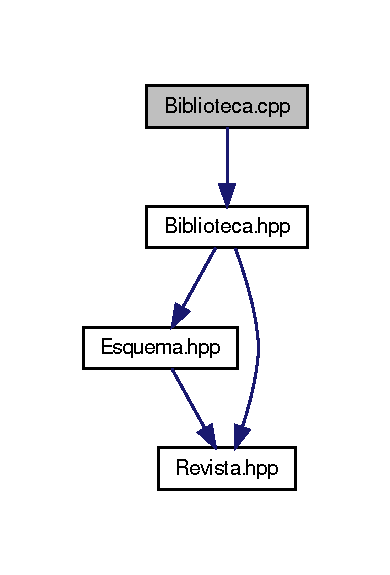
\includegraphics[width=187pt]{_biblioteca_8cpp__incl}
\end{center}
\end{figure}

\hypertarget{_biblioteca_8hpp}{\section{Referencia del Archivo Biblioteca.\-hpp}
\label{_biblioteca_8hpp}\index{Biblioteca.\-hpp@{Biblioteca.\-hpp}}
}


Especificacion de la clase \hyperlink{class_biblioteca}{Biblioteca}.  


Dependencia gráfica adjunta para Biblioteca.\-hpp\-:\nopagebreak
\begin{figure}[H]
\begin{center}
\leavevmode
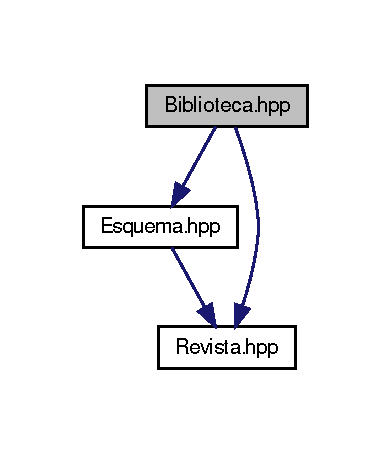
\includegraphics[width=187pt]{_biblioteca_8hpp__incl}
\end{center}
\end{figure}
\subsection*{Clases}
\begin{DoxyCompactItemize}
\item 
class \hyperlink{class_biblioteca}{Biblioteca}
\begin{DoxyCompactList}\small\item\em Representa una coleccion de revistas. \end{DoxyCompactList}\item 
struct \hyperlink{struct_biblioteca_1_1_a1}{Biblioteca\-::\-A1}
\begin{DoxyCompactList}\small\item\em \hyperlink{struct_biblioteca_1_1_a1}{A1} es un struct que contiene por un lado una lista de revistas (L1) y por otro lado una lista de pairs de strings (L2) \end{DoxyCompactList}\end{DoxyCompactItemize}


\subsection{Descripción detallada}
Especificacion de la clase \hyperlink{class_biblioteca}{Biblioteca}. 

Definición en el archivo \hyperlink{_biblioteca_8hpp_source}{Biblioteca.\-hpp}.


\hypertarget{_esquema_8cpp}{\section{Referencia del Archivo Esquema.\-cpp}
\label{_esquema_8cpp}\index{Esquema.\-cpp@{Esquema.\-cpp}}
}
Dependencia gráfica adjunta para Esquema.\-cpp\-:\nopagebreak
\begin{figure}[H]
\begin{center}
\leavevmode
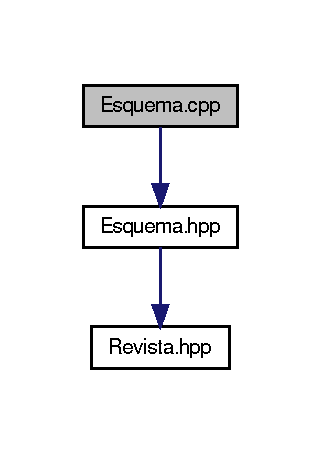
\includegraphics[width=154pt]{_esquema_8cpp__incl}
\end{center}
\end{figure}

\hypertarget{_esquema_8hpp}{\section{Referencia del Archivo Esquema.\-hpp}
\label{_esquema_8hpp}\index{Esquema.\-hpp@{Esquema.\-hpp}}
}


Especificacion de la clase \hyperlink{class_esquema}{Esquema}.  


Dependencia gráfica adjunta para Esquema.\-hpp\-:\nopagebreak
\begin{figure}[H]
\begin{center}
\leavevmode
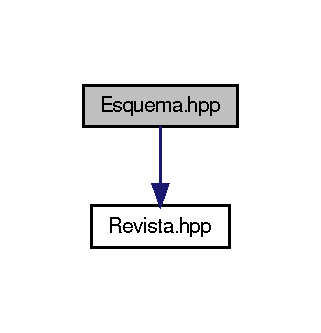
\includegraphics[width=154pt]{_esquema_8hpp__incl}
\end{center}
\end{figure}
\subsection*{Clases}
\begin{DoxyCompactItemize}
\item 
class \hyperlink{class_esquema}{Esquema}
\begin{DoxyCompactList}\small\item\em Representa la organizacion de la coleccion de revistas. \end{DoxyCompactList}\end{DoxyCompactItemize}


\subsection{Descripción detallada}
Especificacion de la clase \hyperlink{class_esquema}{Esquema}. 

Definición en el archivo \hyperlink{_esquema_8hpp_source}{Esquema.\-hpp}.


\hypertarget{pro2_8cpp}{\section{Referencia del Archivo pro2.\-cpp}
\label{pro2_8cpp}\index{pro2.\-cpp@{pro2.\-cpp}}
}
Dependencia gráfica adjunta para pro2.\-cpp\-:\nopagebreak
\begin{figure}[H]
\begin{center}
\leavevmode
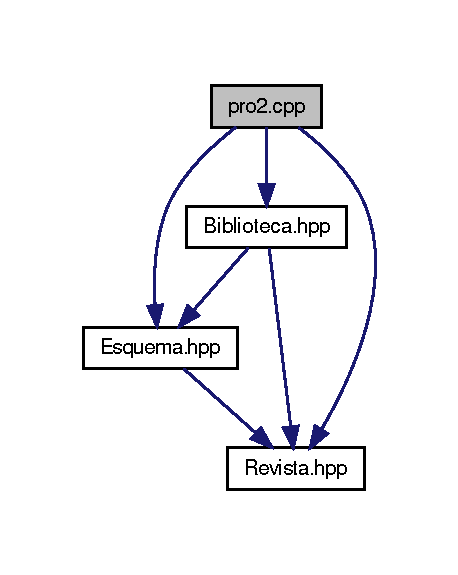
\includegraphics[width=220pt]{pro2_8cpp__incl}
\end{center}
\end{figure}
\subsection*{Funciones}
\begin{DoxyCompactItemize}
\item 
int \hyperlink{pro2_8cpp_ae66f6b31b5ad750f1fe042a706a4e3d4}{main} ()
\end{DoxyCompactItemize}


\subsection{Documentación de las funciones}
\hypertarget{pro2_8cpp_ae66f6b31b5ad750f1fe042a706a4e3d4}{\index{pro2.\-cpp@{pro2.\-cpp}!main@{main}}
\index{main@{main}!pro2.cpp@{pro2.\-cpp}}
\subsubsection[{main}]{\setlength{\rightskip}{0pt plus 5cm}int main (
\begin{DoxyParamCaption}
{}
\end{DoxyParamCaption}
)}}\label{pro2_8cpp_ae66f6b31b5ad750f1fe042a706a4e3d4}


Definición en la línea 5 del archivo pro2.\-cpp.


\begin{DoxyCode}
5           \{
6     \textcolor{keywordtype}{int} N = readint();
7     \hyperlink{class_biblioteca}{Biblioteca} b (N);
8     \hyperlink{class_esquema}{Esquema} e;
9     e.\hyperlink{class_esquema_ad6c7e82a2322bd19412efa51d2005ede}{leer\_esquema}();
10     
11     \textcolor{keywordtype}{int} op;  \textcolor{comment}{//Código de operación}
12     op = readint();
13     \textcolor{keywordflow}{while} (op != -6)\{
14   \textcolor{keywordflow}{if} (op == -1)\{
15       \hyperlink{class_revista}{Revista} r;
16       r.\hyperlink{class_revista_a61178cb7b236db9a3354d5d00df1b31b}{leer\_revista}();
17       \textcolor{keywordtype}{int} calidad = readint();
18       e.\hyperlink{class_esquema_a2a237e94381f752b6f5cb582987b0570}{calcular\_c1}(r);
19       e.\hyperlink{class_esquema_a50c270ca5ba9dbd129fe047fb7a18363}{calcular\_c2}(r);
20       b.alta\_revista(r, calidad);
21   \}
22   \textcolor{keywordflow}{else} \textcolor{keywordflow}{if} (op == -2)\{
23       \textcolor{keywordtype}{string} s = readstring();
24       b.baja\_revista(s);
25   \}
26   \textcolor{keywordflow}{else} \textcolor{keywordflow}{if} (op == -3)\{
27       \textcolor{keywordtype}{string} s1 = readstring();
28       \textcolor{keywordtype}{string} s2 = readstring();
29       \hyperlink{class_revista}{Revista} r1, r2;
30       \textcolor{keywordtype}{int} i1 = 0;
31       \textcolor{keywordtype}{int} i2 = 0;
32       \textcolor{keywordtype}{bool} b1 = \textcolor{keyword}{false};
33       \textcolor{keywordtype}{bool} b2 = \textcolor{keyword}{false};
34       b.consultar\_revista(s1, r1, i1, b1);
35       b.consultar\_revista(s2, r2, i2, b2);
36       b.baja\_revista(s1);
37       b.baja\_revista(s2);
38       r1.\hyperlink{class_revista_a039821163b9175aa556d94b6d7fd6f63}{fusionar\_revista}(r2);
39       e.\hyperlink{class_esquema_a2a237e94381f752b6f5cb582987b0570}{calcular\_c1}(r1);
40       e.\hyperlink{class_esquema_a50c270ca5ba9dbd129fe047fb7a18363}{calcular\_c2}(r1);
41       b.alta\_revista(r1, i1);
42   \}
43   \textcolor{keywordflow}{else} \textcolor{keywordflow}{if} (op == -4)\{
44       \textcolor{keywordtype}{int} calidad = readint();
45       \textcolor{keywordtype}{int} criterio = readint();
46       cout << \textcolor{stringliteral}{"Revistas de calidad "} << calidad << \textcolor{stringliteral}{" por criterio "} << criterio << endl;
47       b.listar\_revistas(calidad, criterio);
48       cout << endl;
49   \}
50   \textcolor{keywordflow}{else} \textcolor{keywordflow}{if} (op == -5)\{
51       cout << \textcolor{stringliteral}{"Consulta de revista por titulo"} << endl;
52       \textcolor{keywordtype}{string} s = readstring();
53       \hyperlink{class_revista}{Revista} r;
54       \textcolor{keywordtype}{bool} b1 = \textcolor{keyword}{false};
55       \textcolor{keywordtype}{int} i = 0;
56       b.consultar\_revista(s, r, i, b1);
57       \textcolor{keywordflow}{if} (b1)\{
58     r.\hyperlink{class_revista_a22abd6f25251e007e5e08bfd11d060a0}{escribir\_revista}();
59     cout << i << endl;
60       \}
61       \textcolor{keywordflow}{else} cout << \textcolor{stringliteral}{"La revista "} << s << \textcolor{stringliteral}{" no existe"} << endl; 
62       cout << endl;
63   \}
64   op = readint();
65     \}
66 \}\end{DoxyCode}

\hypertarget{_revista_8cpp}{\section{Referencia del Archivo Revista.\-cpp}
\label{_revista_8cpp}\index{Revista.\-cpp@{Revista.\-cpp}}
}
Dependencia gráfica adjunta para Revista.\-cpp\-:\nopagebreak
\begin{figure}[H]
\begin{center}
\leavevmode
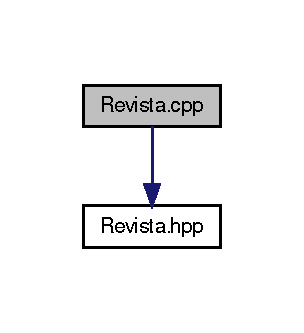
\includegraphics[width=146pt]{_revista_8cpp__incl}
\end{center}
\end{figure}

\hypertarget{_revista_8hpp}{\section{Referencia del Archivo Revista.\-hpp}
\label{_revista_8hpp}\index{Revista.\-hpp@{Revista.\-hpp}}
}


Especificacion de la clase \hyperlink{class_revista}{Revista}.  


\subsection*{Clases}
\begin{DoxyCompactItemize}
\item 
class \hyperlink{class_revista}{Revista}
\begin{DoxyCompactList}\small\item\em Representa el cojunto de caracteristicas y operaciones de las revistas. \end{DoxyCompactList}\end{DoxyCompactItemize}


\subsection{Descripción detallada}
Especificacion de la clase \hyperlink{class_revista}{Revista}. 

Definición en el archivo \hyperlink{_revista_8hpp_source}{Revista.\-hpp}.


%--- End generated contents ---

% Index
\newpage
\phantomsection
\addcontentsline{toc}{part}{Índice}
\printindex

\end{document}
